\subsection{垂直于弦的直径}\label{subsec:czjh2-7-3}

把一张圆形的纸片沿着一条直径对折,可以看到,直径两侧的两个半圆能够互相重合。
这说明圆是轴对称图形,而直径所在的直线就是它的对称轴。下面我们来证明这个结论。

\begin{wrapfigure}[9]{r}{4.5cm}
    \centering
    \begin{tikzpicture}
    \tkzDefPoints{0/0/O}
    \tkzDefPoint(90:1.5){C}
    \tkzDefPoint(270:1.5){D}
    \tkzDefPoint(230:1.5){A}
    \tkzDefLine[perpendicular=through A](C,D)  \tkzGetPoint{a}
    \tkzInterLC[common=A](A,a)(O,A)  \tkzGetFirstPoint{A'}
    \tkzInterLL(A,A')(C,D)  \tkzGetPoint{M}

    \tkzDrawCircle[thick](O,A)
    \tkzDrawLine[add=0.2 and 0.2](C,D)
    \tkzDrawSegment(A,A')
    \tkzDrawSegments[dashed](O,A  O,A')
    \tkzMarkRightAngle(A',M,C)
    \tkzDrawPoint(O)
    \tkzLabelPoints[left,xshift=-.3em](A)
    \tkzLabelPoints[right](A', O)
    \tkzLabelPoints[above left](C)
    \tkzLabelPoints[below left](D)
    \tkzLabelPoints[above, xshift=-.6em](M)
\end{tikzpicture}


    \caption{}\label{fig:czjh2-7-11}
\end{wrapfigure}

如图 \ref{fig:czjh2-7-11}, 设 $CD$ 是 $\yuan\,O$ 的任意一条直径,$A$ 为 $\yuan\,O$ 上任意一点。
过点 $A$ 作 $AA' \perp CD$, 交 $\yuan\,O$ 于点 $A'$,垂足为 $M$。连结 $OA$、$OA'$。

在 $\triangle AOA'$ 中,

$\because$ \quad $OA = OA'$, $AA' \perp CD$,

$\therefore$ \quad $AM = MA'$。

即 $CD$ 是 $AA'$ 的垂直平分线,这就是说,对于圆上任意一点 $A$,
在圆上都有关于直线 $CD$ 的对称点 $A'$,因此 $\yuan\,O$ 关于 $CD$ 对称。即

\begin{xingzhi}
    圆是轴对称图形,经过圆心的每一条直线都是对称轴。
\end{xingzhi}

从上面的证明,我们知道,如果 $AA' \perp CD$,那么点 $A$ 和 $A'$ 是对称点,
所以 $AM$ 和 $A'M$、$\yuanhu{AD}$ 和 $\yuanhu{A'D}$ 能够互相重合。于是有下面定理:

\begin{dingli}[垂径定理]
    垂直于弦的直径平分这条弦,并且平分弦所对的弧。
\end{dingli}

由垂径定理,可以推出下面的推论:

\begin{tuilun}[推论1]
    (1)平分弦(不是直径)的直径垂直于弦,并且平分弦所对的弧;
    (2)平分弦所对的一条弧的直径,垂直平分弦;
    (3)弦的垂直平分线经过圆心,并平分弦所对的弧。
\end{tuilun}

\begin{tuilun}[推论2]
    圆的两条平行弦所夹的弧相等。
\end{tuilun}

如图 \ref{fig:czjh2-7-12} 中, $AB \pingxing CD$, 则 $\yuanhu{AC} = \yuanhu{BD}$。

\begin{figure}[htbp]
    \centering
    \begin{minipage}[b]{7cm}
        \centering
        \begin{tikzpicture}
    \tkzDefPoints{0/0/O}
    \tkzDefPoint(90:1.5){M}
    \tkzDefPoint(270:1.5){N}
    \tkzDefPoint(160:1.5){A}
    \tkzDefPoint(20:1.5){B}
    \tkzDefPoint(130:1.5){C}
    \tkzDefPoint(50:1.5){D}

    \tkzDrawCircle[thick](O,A)
    \tkzDrawSegments(M,N  A,B  C,D)
    \tkzDrawPoint(O)
    \tkzLabelPoints[left](A,C)
    \tkzLabelPoints[right](B,D,O)
    \tkzLabelPoints[above](M)
    \tkzLabelPoints[below](N)
\end{tikzpicture}


        \caption{}\label{fig:czjh2-7-12}
    \end{minipage}
    \qquad
    \begin{minipage}[b]{7cm}
        \centering
        \begin{tikzpicture}
    \tkzDefPoints{0/0/O}
    \tkzDefPoint(160:1.5){A}
    \tkzDefPoint(20:1.5){B}
    \tkzDrawArc[thick](O,B)(A)
    \tkzLabelPoints[left](A)
    \tkzLabelPoints[right](B)

    % 1
    \tkzDrawSegment(A,B)

    % 2
    \tkzDefLine[mediator,K=.7](A,B)  \tkzGetPoints{C}{D}
    \tkzInterLC(C,D)(O,A)  \tkzGetFirstPoint{E}
    \tkzCompasss(A,C  B,C  A,D  B,D)
    \tkzDrawLine[add=0.1 and 0.1](C,D)
    \tkzDrawPoint(E)
    \tkzLabelPoints[right](C,D)
    \tkzLabelPoints[above right](E)
\end{tikzpicture}


        \caption{}\label{fig:czjh2-7-13}
    \end{minipage}
\end{figure}

\liti 平分已知 $\yuanhu{AB}$。

已知: $\yuanhu{AB}$(图 \ref{fig:czjh2-7-13})。

求作:$\yuanhu{AB}$ 的中点。

\zuofa 1. 连结 $AB$。

2. 作 $AB$ 的垂直平分线 $CD$,交 $\yuanhu{AB}$ 于点 $E$。

点 $E$ 就是所求 $\yuanhu{AB}$ 的中点。

证明略。


\liti 一千三百多年前,我国隋代建造的赵州石拱桥(图 \ref{fig:czjh2-7-14})的桥拱是圆弧形,
它的跨度(弧所对的弦的长)为 37.4 米,拱高(弧的中点到弦的距离,也叫弓形高)为7.2米,
求桥拱的半径(精确到 0.1 米)。

\begin{figure}[htbp]
    \centering
    \begin{minipage}[b]{10.5cm}
        \centering
        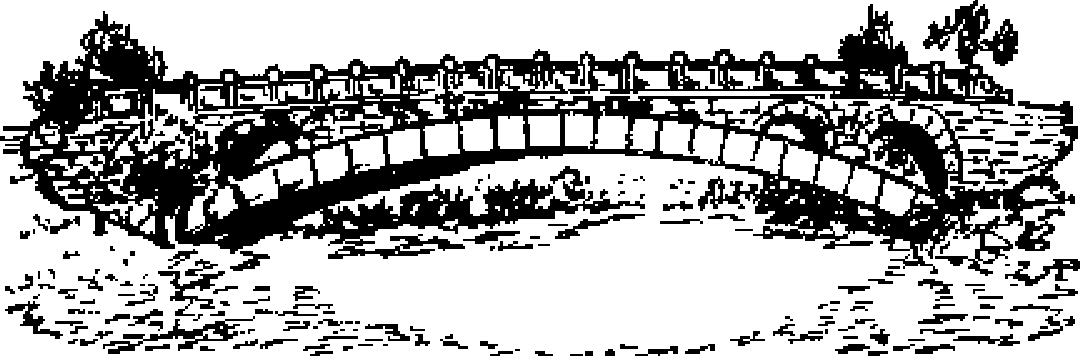
\includegraphics[width=10cm]{../pic/czjh2-ch7-14.png}
        \caption{}\label{fig:czjh2-7-14}
    \end{minipage}
    \qquad
    \begin{minipage}[b]{5cm}
        \centering
        \begin{tikzpicture}[>=Stealth,]
    \pgfmathsetmacro{\factor}{0.1}
    \tkzDefPoints{0/0/O}
    \tkzDefPoint(90:27.9*\factor){C}
    \tkzDefPointOnLine[pos=7.2/37.4](C,O)  \tkzGetPoint{D}
    \tkzDefLine[perpendicular=through D](O,C)  \tkzGetPoint{a}
    \tkzInterLC(D,a)(O,C)  \tkzGetPoints{B}{A}

    \tkzDrawArc[thick](O,B)(A)
    \tkzDrawSegments[dashed](O,C A,B B,O O,A)
    \tkzMarkRightAngle[size=0.2](A,D,O)
    \tkzLabelSegment[below left](O,A){$R$}
    \tkzLabelPoints[below,xshift=-.3em](A)
    \tkzLabelPoints[below right](B)
    \tkzLabelPoints[below right](C)
    \tkzLabelPoints[below right](D)
    \tkzLabelPoints[below](O)

    %
    \tkzDefPointBy[translation=from D to C](A)  \tkzGetPoint{E}
    \tkzDefShiftPoint[A](-0.5,0){Ha}
    \tkzDefPointBy[translation=from A to Ha](E)  \tkzGetPoint{He}
    \tkzDefShiftPoint[Ha](0,-0.3){Has}
    \tkzDefShiftPoint[He](0, 0.3){Hes}
    \tkzDrawLine[add=0 and 0.4](A,Ha)  \tkzDrawSegments(C,E)
    \tkzDrawLine[add=0 and 0.4](E,He)
    \tkzDrawSegment[-latex](Has,Ha)
    \tkzDrawSegment[-latex](Hes,He)
    \tkzLabelSegment[rotate=90,yshift=.5em](Ha,He){\footnotesize $7.2$}

    \tkzDefShiftPoint[A](0, 0.9){Wa}
    \tkzDefShiftPoint[B](0, 0.9){Wb}
    \tkzDrawLines[add=0 and 0.3](A,Wa  B,Wb)
    \tkzDrawSegment[latex-latex](Wa,Wb)
    \tkzLabelSegment[yshift=.5em,fill=white, inner sep=1pt](Wa,Wb){$37.4$}
    % \draw [latex-latex] (Wa) to [xianduan] node [fill=white, inner sep=1pt]{$30$} (Wb);
    % \tkzDrawSegment[dim={$37.4$,10pt,}](Wa,Wb)
\end{tikzpicture}


        \caption{}\label{fig:czjh2-7-15}
    \end{minipage}
\end{figure}

\jie 如图 \ref{fig:czjh2-7-15}, 用 $\yuanhu{AB}$ 表示桥拱, $\yuanhu{AB}$ 的圆心为 $O$、半径为 $R$ 米。
经过圆心 $O$ 作弦 $AB$ 的垂线 $OD$, $D$为垂足, 与 $\yuanhu{AB}$ 相交于点 $C$。
根据垂径定理, $D$ 是 $AB$ 的中点, $C$ 是 $\yuanhu{AB}$ 的中点, $CD$ 就是拱高。由题设
\begin{gather*}
    AB = 37.4 \douhao  CD = 7.2 \douhao \\
    AD = \exdfrac{1}{2} AB = \exdfrac{1}{2} \times 37.4 = 18.7 \douhao \\
    OD = OC - DC = R - 7.2 \juhao
\end{gather*}

在 $Rt \triangle OAD$ 中,由勾股定理,得
$$ OA^2 = AD^2 + OD^2 \douhao $$

即 $R^2 = 18.7^2 + (R - 7.2)^2 \juhao $

解这个方程,得 $R \approx 27.9$(米)。

答: 赵州石拱桥的桥拱半径约为 27.9 米。


\begin{lianxi}

\xiaoti{(口答)}%
\begin{xiaoxiaotis}%
    \xxt[-1em]{平分一条弧的直径有什么性质?}

    \xxt{平分弦和它所对的一条弧的直线有什么性质?}

    \xxt{垂直弦,并平分弦所对的一条弧的直线有什么性质?}

\end{xiaoxiaotis}

\xiaoti{在平径为 50 mm 的 $\yuan\,O$ 中, 有长 50 mm 的弦 $AB$。计算:}
\begin{xiaoxiaotis}

    \xxt{点 $O$ 与 $AB$ 的距离;}

    \xxt{$\angle AOB$ 的度数。}

\end{xiaoxiaotis}

\xiaoti{以点 $O$ 为圆心的两个同心圆中,大圆的弦 $AB$ 和小圆相交于点 $C$ 和 $D$。
    求证: $AC = BD$。
}

\end{lianxi}

